\chapter{Discussion}\label{ch:discussion}
In chapter \ref{ch:problem_description},
specific success criteria were created to
limit the scope and also allow for the project to be 
evaluated. 
This discussion will focus on what was accomplished
in terms of success criteria and on the possible
future steps to improve or advance this project.
The list of success criteria from Section \ref{sec:PD} 
is shown below:
\begin{itemize}
    \item Data mining
    \item Choose a filter
    \item Design a deep neural network model
    \item Train for the English language
    \item Create a Client/Server framework
    \item Implement the distributed model
\end{itemize} 
In order to use the OpenSLR training set,
it was crucial to develop and use the scripts
detailed in Section\ref{sec:DataMining}.
Having an algorithm capable of following a path
from a main folder and its sub-folders to
convert all the necessary files to the right
format meant that the amount of data increased drastically.
Using up to $1000$ hours of speech for the neural
network to learn from was crucial in the development
phase.
As no neural network, no matter how complex and
well thought out, could have a scope of
understanding the full English language from a
limited data set. 
Another important difference is to be made between
clean speech and noisy speech, as a network
trained only with clean speech stands no chance
of recognizing our voices.
The preprocessing part covered in Chapter 
\ref{ch:speech_processing}, more specifically in Section 
\ref{sec:Modernanalysis}, was successfully implemented 
by using the 26 cepstrum coefficient to shape 
information to be fed to the first layer of neurons. 
With the MFCC, the signal used as an input is converted 
to the frequency domain and distributed evenly on a 
scale mimicking the human ear. Without this step, the 
neural network wouldn't have been able to
receive any input.\\\\
For the main part, which consisted of the design and 
development of the neural network model, a reference 
model was originally used for understanding and testing. 
The silicon-valley-data-science model with the simple 
LSTM neural network proved to be a strong starting point 
for our own neural networks. As it was used to get 
acquainted with all the different dependencies and 
intricacies that these systems possess.
By reverse engineering the reference model,
we were able to construct a series of more complex
and better-performing networks.\\\\ 
By trial and error, the first fully functional model 
that outperformed the silicon-valley-data-science model 
was described in Section \ref{sec:NNComparison}.
The addition of fully connected layers both before
and after the core LSTM layers proved to be an
efficient way of reducing the word error rate across
all the testing range, clearly seen in Figure 
\ref{fig:validation_error_fig}.
A further analysis of the state-of-the-art neural 
networks developed specifically for understanding
speech revealed that a BiRNN could prove to be a better 
solution to the classical stacking of LSTM layers.
From the idea that hidden vectors can compute
previous and future states, a second model was pursued,
having a BiRNN layer as its core.
Seen in Figure \ref{fig:BiRNNFC}, the best performing 
model is shown as a combination of FC and BiRNN.\\\\
Both models, LSTM and BiRNN were trained in the English 
language, by using the LibriSpeech set.
To achieve this goal, a large number of parameters had 
to be tuned to ensure that the network didn't diverge 
during learning.
As there is no predetermined way to set the parameters, 
training was done on an iterative process and the 
results were documented in Appendix
\ref{ch:appClabel}.\\\\
The next step was to distribute the speech recognition 
(SR) system.
The server was established on the computer which
had the video card and where the neural
network was designed.
This was done in order to assure that the server had
enough processing power to complete the tasks sent by
the users.
Via the LAN network, any client that has access
to the SR system can send a .wav
file and receive a written text file containing the
transcription of their voice.
\section{Future Work}
For future development, a series of topics can
be pursued for the betterment of the DSR system.
One of the key ideas pointed out in the report was
that training data is crucial for the system, and as 
such, a first addition should constitute in the
creation of even larger datasets. 
While a larger set of data will prove beneficial,
sets that emulate real-life speech, such as speech
in a noisy environment or multiple speakers at the
same time will greatly benefit the learning curve
of any neural network.
The scope of this project was also limited by the 
hardware available at the time of this research paper,
with such considerations, more powerful hardware will 
prove instrumental in reducing the processing time and 
increasing the efficiency of writing and developing 
better neural networks.
Due to time constraints, a balance between the time
that the network was training and time the models
were developed had to be maintained.
Moreover, data sets should be able to run for
increased amounts of time to reduce the word error rate 
even further.\\\\
A major goal that can be achieved by building upon the
results of this project is the creation of an
information retrieval (IR) system.
As data is returned in text format to the client,
an IR system can search a predefined database,
or use a web crawler to access specific web pages
and return meaningful snippets of information
related to the predetermined interests of the user.\\\\
Another improvement would target the distribution part 
of the system.
TensorFlow Serving is a flexible, high-performance 
serving system for machine learning models.
It is designed for production environments,
and it provides an easy way to deploy new algorithms
and experiments, without changing the server 
architecture, illustrated in \ref{fig:TFServe}.
It would provide a great option for testing different 
models efficiently.
\begin{figure}[H]
    \centering
    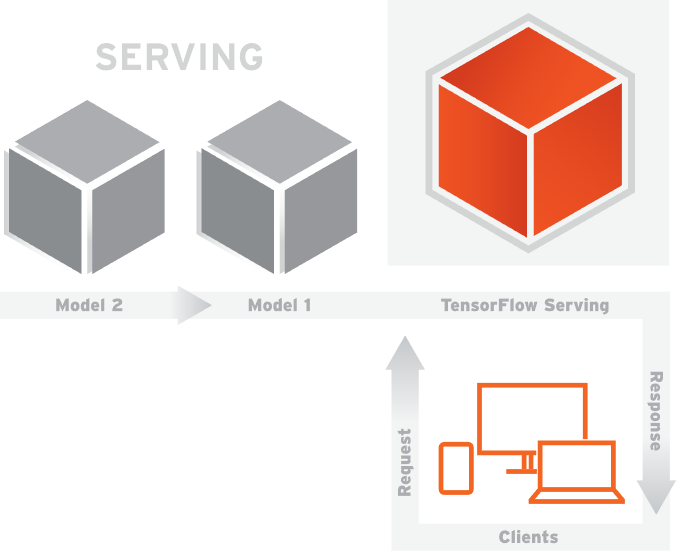
\includegraphics[width=.7\textwidth]        
    {future_work/TensorFlowServing}
    \caption{TensorFlow Serving \cite{TFServ}.}
    \label{fig:TFServe}
\end{figure}